%% ============================================================
%%  SECTION 3 — DỮ LIỆU & BÀI TOÁN BAN ĐẦU  (số liệu: v2)
%%  Data Pipeline: thu thập → tích hợp → làm sạch → EDA → Final Data
%% ============================================================
\section{Dữ liệu và Bài toán ban đầu}
\label{sec:data}

\subsection{Lý do chọn bộ dữ liệu}

Không có bộ dữ liệu cho thuê đa nguồn sẵn có ở Việt Nam,
nên nhóm tự thu thập bằng \textbf{web scraping} từ 10 nguồn khác nhau.
Lý do chọn cách này:
\begin{itemize}[leftmargin=*, itemsep=2pt]
  \item Bao phủ nhiều phân khúc thị trường (từ phòng trọ bình dân tới căn hộ).
  \item Đảm bảo tính đại diện địa lý (Hà Nội, TP.HCM, Đà Nẵng và 16 tỉnh thành khác).
  \item Có thể kiểm soát chất lượng và schema từ đầu, thay vì phụ thuộc nguồn
        bên thứ ba có thể thay đổi.
\end{itemize}

\subsection{Thu thập dữ liệu (Web Scraping)}
\label{subsec:collection}

\begin{table}[H]
  \centering
  \caption{Phân bố bản ghi theo nguồn dữ liệu (sau làm sạch)}
  \label{tab:sources}
  \begin{tabular}{@{}lrr@{}}
    \toprule
    \textbf{Nguồn} & \textbf{Số bài} & \textbf{Tỷ lệ} \\
    \midrule
    chothuephongtro     & 95.086 & \textbf{71.2\%} \\
    nhatot              &  9.920 & 7.4\% \\
    chothuenhadattoanvn &  9.866 & 7.4\% \\
    github\_hcm         &  8.771 & 6.6\% \\
    github\_hn          &  2.879 & 2.2\% \\
    phongtro123         &  2.663 & 2.0\% \\
    github\_housing     &  1.635 & 1.2\% \\
    lozido              &  1.313 & 1.0\% \\
    facebook            &    772 & 0.6\% \\
    github\_dn          &    681 & 0.5\% \\
    \midrule
    \textbf{Tổng} & \textbf{133.586} & \textbf{100\%} \\
    \bottomrule
  \end{tabular}
\end{table}

\begin{figure}[H]
  \centering
  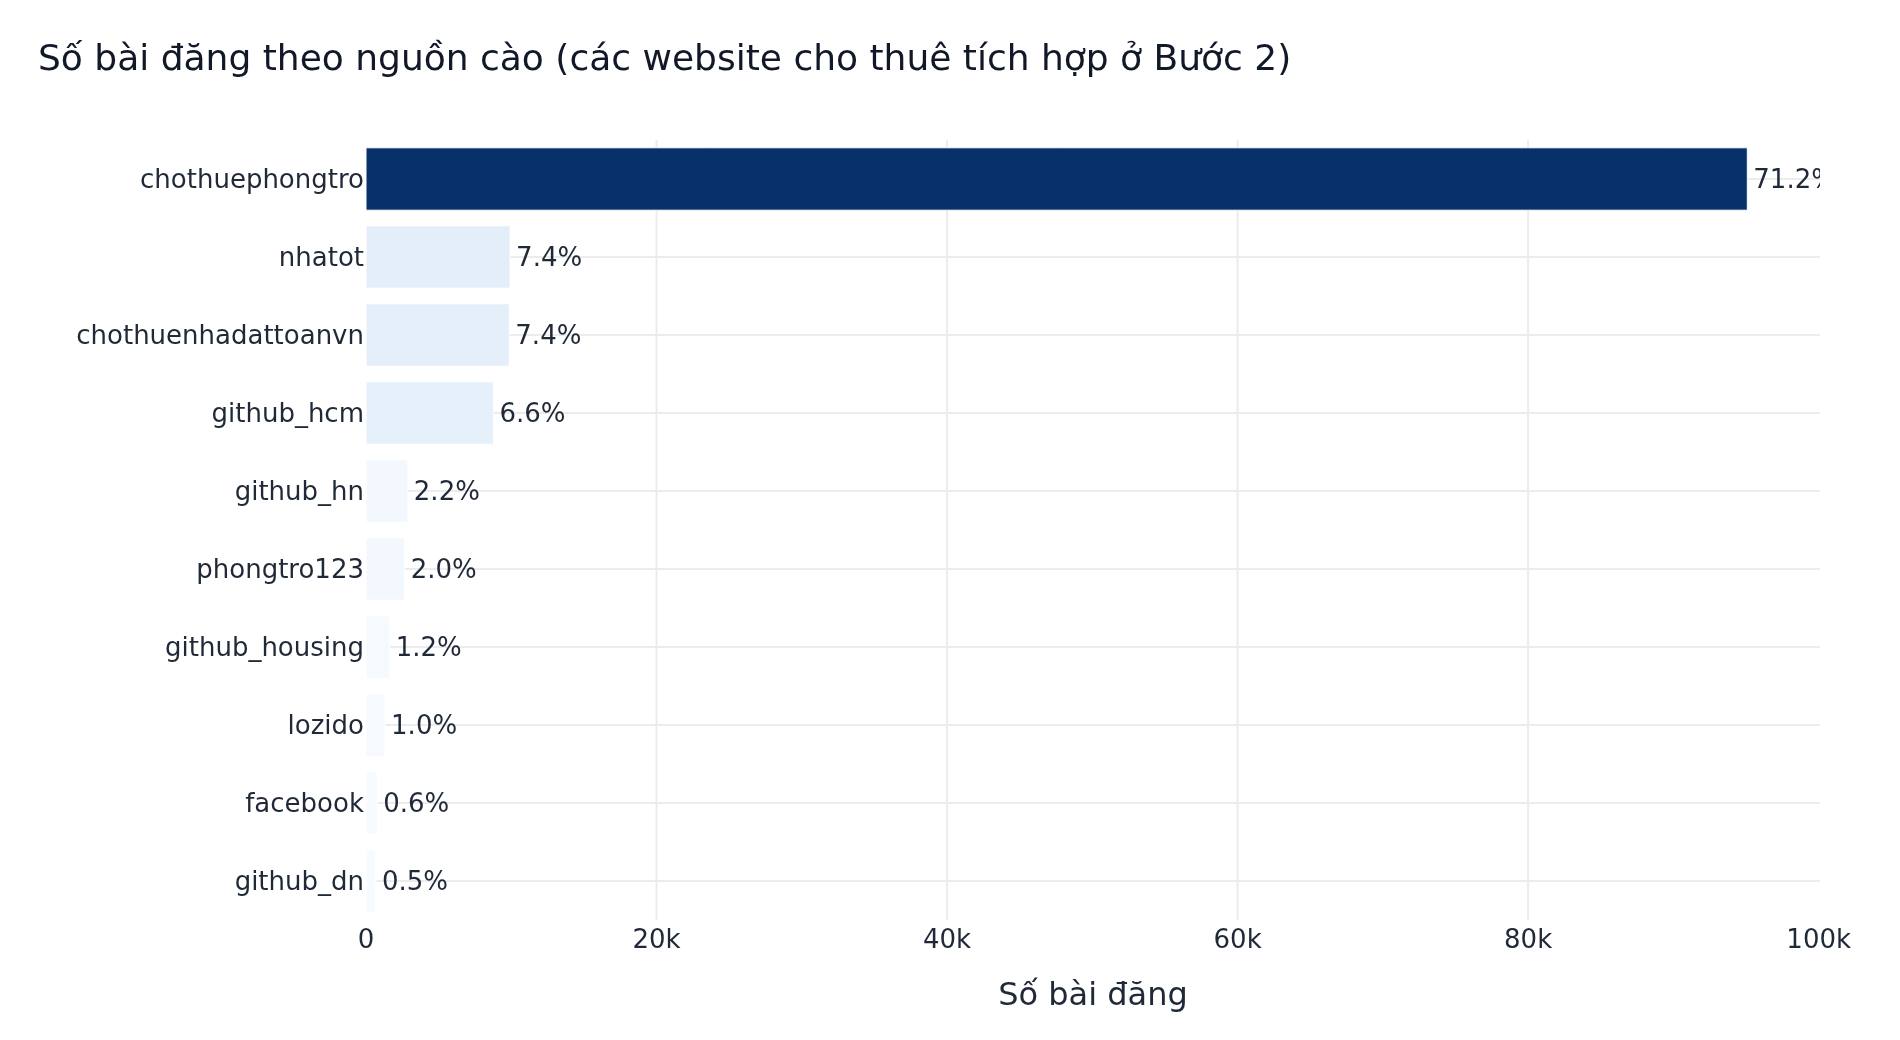
\includegraphics[width=0.86\textwidth]{eda_01_source_distribution}
  \caption{Phân bố bản ghi theo nguồn — \texttt{chothuephongtro} chiếm 71.2\%
           (mất cân bằng nghiêm trọng, quyết định loại \texttt{source} khỏi đặc trưng mô hình,
           xem Mục~\ref{subsec:simpson})}
  \label{fig:source_dist}
\end{figure}

\subsection{Tích hợp và lược đồ chung}
\label{subsec:schema}

Để hợp nhất 10 nguồn có định dạng khác nhau, nhóm thiết kế
\textbf{lược đồ thống nhất} (mediated schema) với các trường:
\texttt{price, area, bedrooms, bathrooms, full\_address, posted\_date, source}
cùng 12 cờ nhị phân \texttt{feature\_*}.
Quy trình ETL gồm bốn bước:
\begin{itemize}[leftmargin=*, itemsep=2pt]
  \item Chuẩn hóa giá và diện tích từ chuỗi văn bản về số (biểu thức chính quy).
  \item Loại tin \texttt{price = -1} (\textit{``giá thỏa thuận''}).
  \item Khử trùng lặp; mã hóa one-hot 12 tiện ích.
  \item \textbf{Lọc ngoại lệ:} \texttt{price}$\leq$17 triệu/tháng;
        \texttt{area}$\leq$180 m\textsuperscript{2}
        (ngưỡng chọn từ phân tích EDA, đúng phạm vi nhà trọ/căn hộ bình dân).
\end{itemize}

\subsection{Chất lượng dữ liệu và xử lý ngoại lệ (Outlier)}
\label{subsec:quality}

\begin{table}[H]
  \centering
  \caption{Các vấn đề chất lượng dữ liệu và cách xử lý}
  \label{tab:quality}
  \begin{tabularx}{\textwidth}{@{}L{3.0cm} L{5.2cm} X@{}}
    \toprule
    \textbf{Vấn đề} & \textbf{Phát hiện} & \textbf{Xử lý \& lý do} \\
    \midrule
    Ngoại lệ cực đoan &
      Giá tới 10.000 triệu/tháng ($\approx$10 tỷ); diện tích tới 1.000 m\textsuperscript{2} &
      Lọc \texttt{price}$\leq$17; \texttt{area}$\leq$180 — ngoại lệ kéo lệch
      hàm mất mát bình phương, làm mô hình phân bổ năng lực sai vùng giá
      (xác nhận bằng thực nghiệm~\ref{subsec:abl_outlier}) \\
    \addlinespace
    Giá trị thiếu &
      \texttt{detail\_link} 96.4\%;\newline
      \texttt{description} 80.4\%;\newline
      \texttt{district} 2.2\% (2.938 dòng) &
      Loại hai cột thiếu nhiều;\newline
      \texttt{district} thiếu $\to$ gán nhãn \textit{(không rõ)} \\
    \addlinespace
    Sentinel ngày &
      \texttt{posted\_date}: \textbf{46\%} bản ghi mang ngày tương lai &
      Không dùng \texttt{posted\_date} trong mô hình \\
    \addlinespace
    Cờ tiện ích chế tác &
      Kiểm toán raw$\leftrightarrow$hợp nhất (Mục~\ref{subsec:audit}): chỉ \textbf{5/12 cờ}
      có cột gốc thật ở đa số nguồn; 7 cờ còn lại bị \textbf{điền ngẫu nhiên} khi gộp
      ($\approx$97\% số dòng) &
      Mask các ô chế tác thành NaN theo cơ chế MNAR
      (``không khai báo'' $\neq$ ``không có'');
      loại \texttt{n\_features} khỏi đặc trưng \\
    \addlinespace
    Miền giá trị &
      Sau lọc: \texttt{price} 0.5--17;\quad \texttt{area} 8--180 &
      Hợp lệ, không cần xử lý thêm \\
    \bottomrule
  \end{tabularx}
\end{table}

\subsection{Phân tích khám phá dữ liệu (EDA)}
\label{subsec:eda}

\subsubsection*{Thống kê mô tả (Phân tích đơn biến)}

\begin{table}[H]
  \centering
  \caption{Thống kê mô tả các biến liên tục ($n = 133.586$, sau lọc ngoại lệ)}
  \label{tab:descriptive}
  \small
  \begin{tabular}{@{}lrrrrrrr@{}}
    \toprule
    \textbf{Biến} &
    \textbf{Mean} & \textbf{Std} & \textbf{Min} &
    \textbf{Median} & \textbf{Max} &
    \textbf{Skew} & \textbf{Kurt} \\
    \midrule
    \texttt{price} (tr.đ/tháng)
      & 4.80 & 2.87 & 0.5 & 4.00 & 17.0 & \textbf{1.55} & 2.46 \\
    \texttt{area} (m\textsuperscript{2})
      & 41.48 & 27.72 & 8.0 & 30.00 & 180.0 & \textbf{1.59} & 2.35 \\
    \texttt{bedrooms}
      & 1.51 & 0.98 & 0 & 1 & 6 & 2.08 & 4.45 \\
    \texttt{bathrooms}
      & 1.29 & 0.73 & 0 & 1 & 5 & 2.89 & 9.91 \\
    \texttt{n\_features}
      & 6.56 & 1.94 & 0 & 7 & 12 & $-$0.12 & $-$0.20 \\
    \bottomrule
  \end{tabular}
\end{table}

\textbf{Ý nghĩa ra quyết định:}
\texttt{price} và \texttt{area} lệch phải rõ rệt (skewness $\approx$ 1.5--1.6).
Phân phối lệch gợi ý thử log-transform; tuy nhiên thực nghiệm đối sánh
(Mục~\ref{subsec:abl_log}) cho thấy log \textbf{không} cải thiện chỉ số chính RMSE/R\textsuperscript{2}
và gây underweight phân khúc giá cao — do đó mô hình huấn luyện trên \texttt{price} gốc.

\begin{figure}[H]
  \centering
  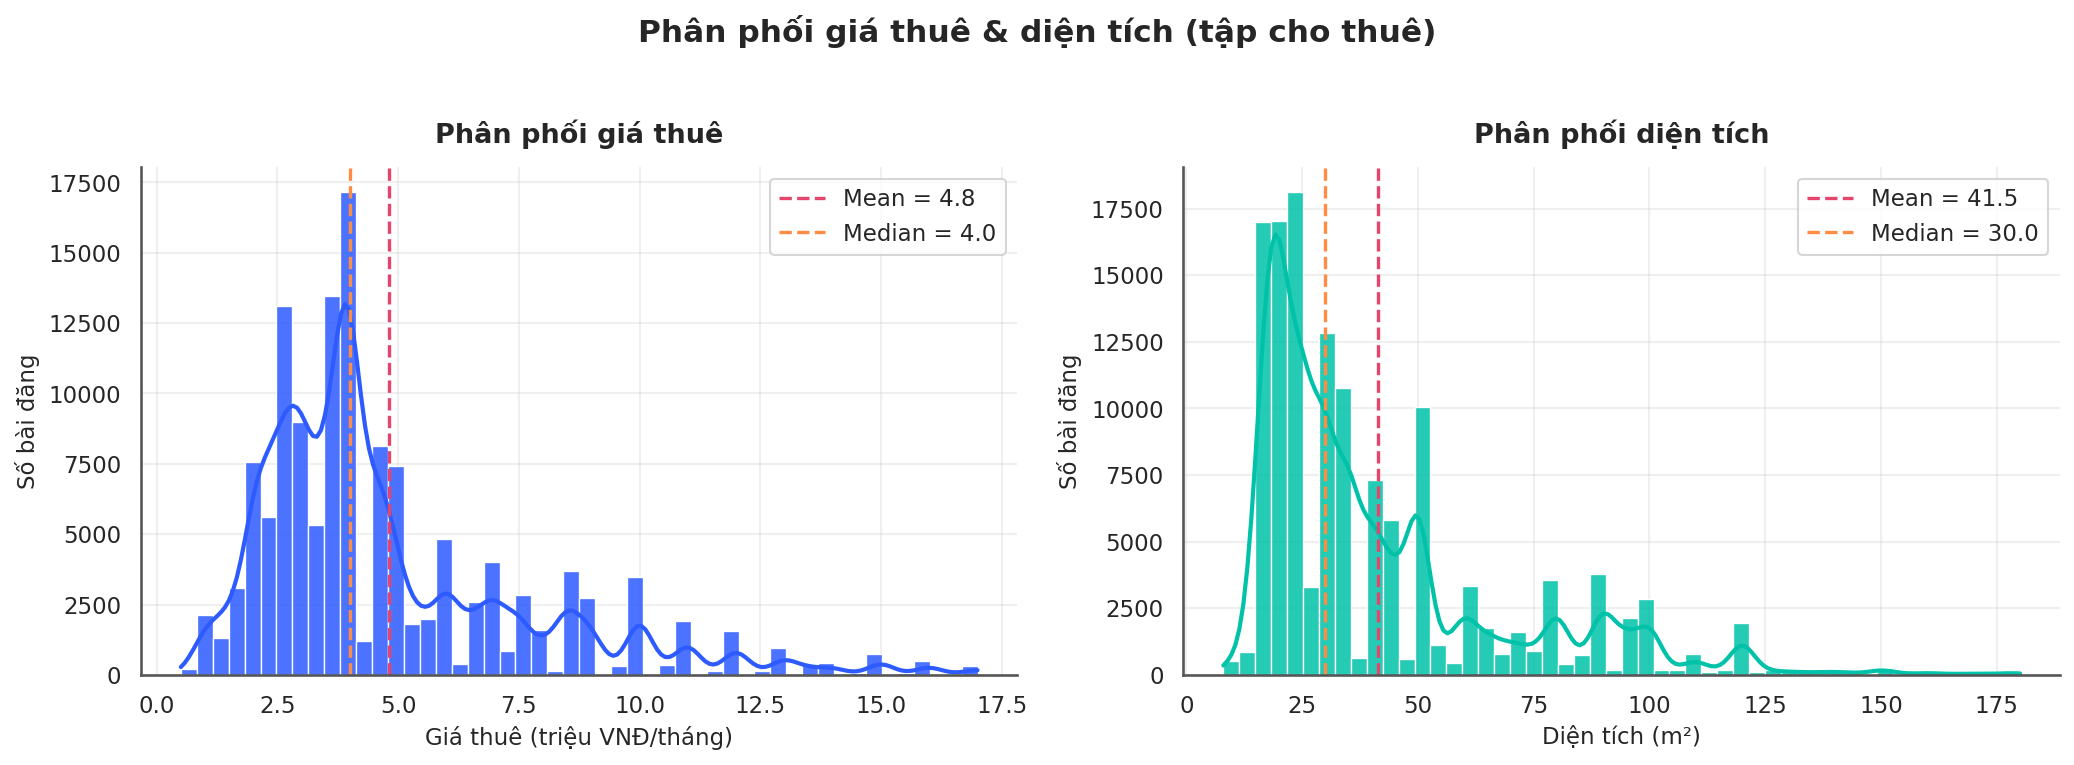
\includegraphics[width=0.86\textwidth]{eda_02_histogram_price_area}
  \caption{Phân phối \texttt{price} và \texttt{area} — cả hai lệch phải rõ rệt;
           phần lớn phòng có diện tích 20--60 m\textsuperscript{2} và giá 2--8 triệu/tháng}
  \label{fig:hist}
\end{figure}

\subsubsection*{Phân bố địa lý}

\begin{table}[H]
  \centering
  \caption{Phân bố địa lý — tập trung nặng tại Hà Nội (88\%)}
  \label{tab:geo}
  \begin{tabular}{@{}lrr@{}}
    \toprule
    \textbf{Thành phố} & \textbf{Số bài} & \textbf{Tỷ lệ} \\
    \midrule
    Hà Nội        & 117.574 & \textbf{88.0\%} \\
    Hồ Chí Minh  &  11.559 & 8.7\% \\
    Đà Nẵng      &   1.411 & 1.1\% \\
    Các tỉnh khác & $<1\%$ mỗi tỉnh & --- \\
    \bottomrule
  \end{tabular}
\end{table}

\textbf{Ý nghĩa ra quyết định:} mất cân bằng địa lý mạnh (88\% là Hà Nội).
Khi dùng One-Hot Encoding cho \texttt{district} (353 giá trị), nhiều quận tỉnh lẻ
có rất ít mẫu $\to$ cần gộp hạng mục hiếm (\texttt{min\_frequency=100}) để
tránh bùng nổ chiều và đảm bảo mô hình xử lý được hạng mục lạ lúc dự đoán.

\subsubsection*{Phân tích đa biến và tương quan}

\begin{table}[H]
  \centering
  \caption{Tương quan Spearman giữa các đặc trưng và \texttt{price}}
  \label{tab:spearman}
  \begin{tabular}{@{}lr@{}}
    \toprule
    \textbf{Biến} & \textbf{Spearman với \texttt{price}} \\
    \midrule
    \texttt{area}        & $\mathbf{+0.366}$ \\
    \texttt{bathrooms}   & $+0.141$ \\
    \texttt{bedrooms}    & $+0.115$ \\
    \texttt{n\_features} &
      $\mathbf{-0.119}$\quad\textit{(phản trực giác — xem Mục~\ref{subsec:simpson})} \\
    \bottomrule
  \end{tabular}
\end{table}

\begin{figure}[H]
  \centering
  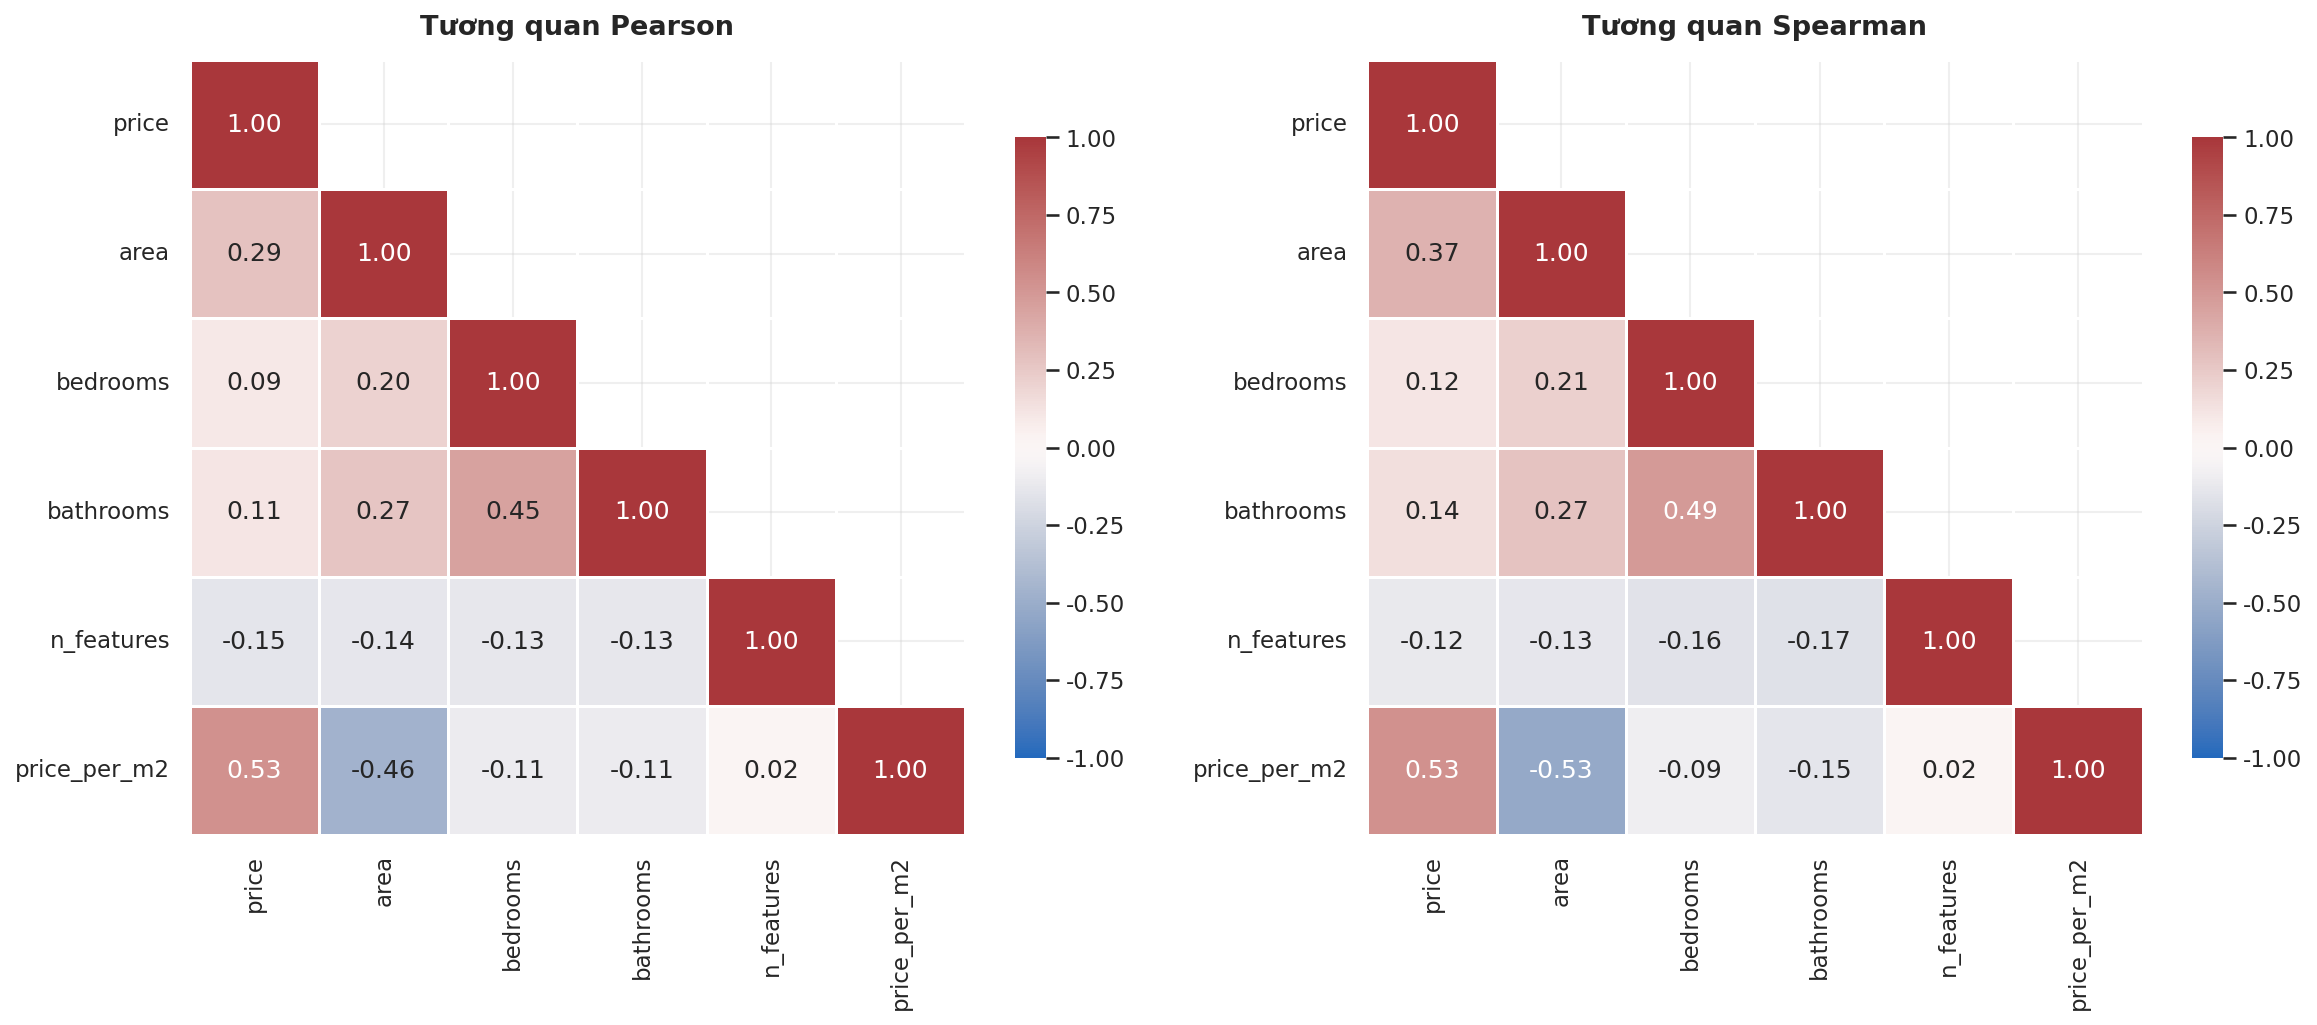
\includegraphics[width=0.76\textwidth]{eda_11_heatmap_correlation}
  \caption{Heatmap tương quan Spearman — \texttt{area} tương quan mạnh nhất với giá;
           tương quan \texttt{n\_features}--\texttt{price} âm là tín hiệu cần điều tra}
  \label{fig:heatmap}
\end{figure}

\begin{figure}[H]
  \centering
  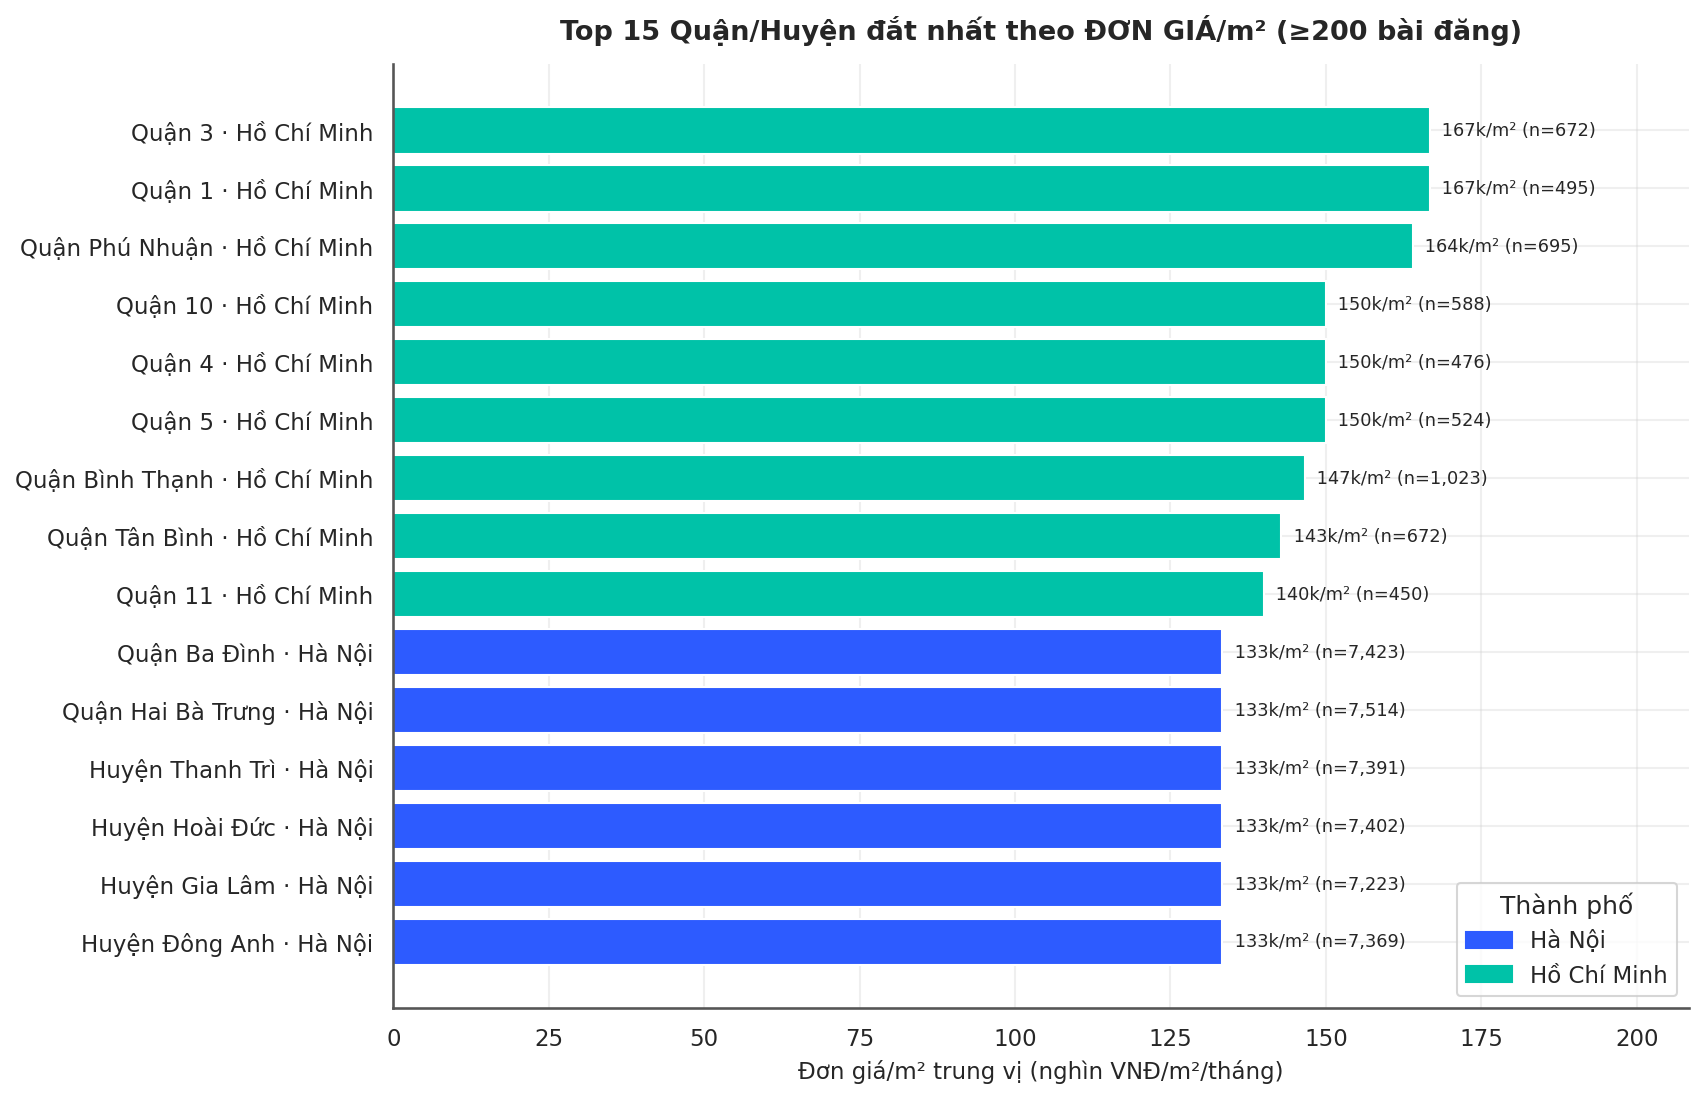
\includegraphics[width=0.86\textwidth]{eda_05_price_per_m2_ranking}
  \caption{Top quận/huyện theo đơn giá thuê — trung tâm TP.HCM (Quận 1, 3) đắt nhất;
           kết quả này thúc đẩy việc tách \texttt{city}/\texttt{district} làm đặc trưng chính}
  \label{fig:price_ranking}
\end{figure}

\subsection{Nghịch lý Simpson — phát hiện quan trọng}
\label{subsec:simpson}

\subsubsection*{Hiện tượng phản trực giác}

Khi so sánh giá trung bình giữa nhóm ``có tiện ích'' và ``không có'',
phần lớn tiện ích đi kèm với giá \textbf{thấp hơn} (bảo vệ 24/24: $-1.44$ triệu;
hầm để xe: $-1.01$; máy lạnh: $-0.73$):

\begin{figure}[H]
  \centering
  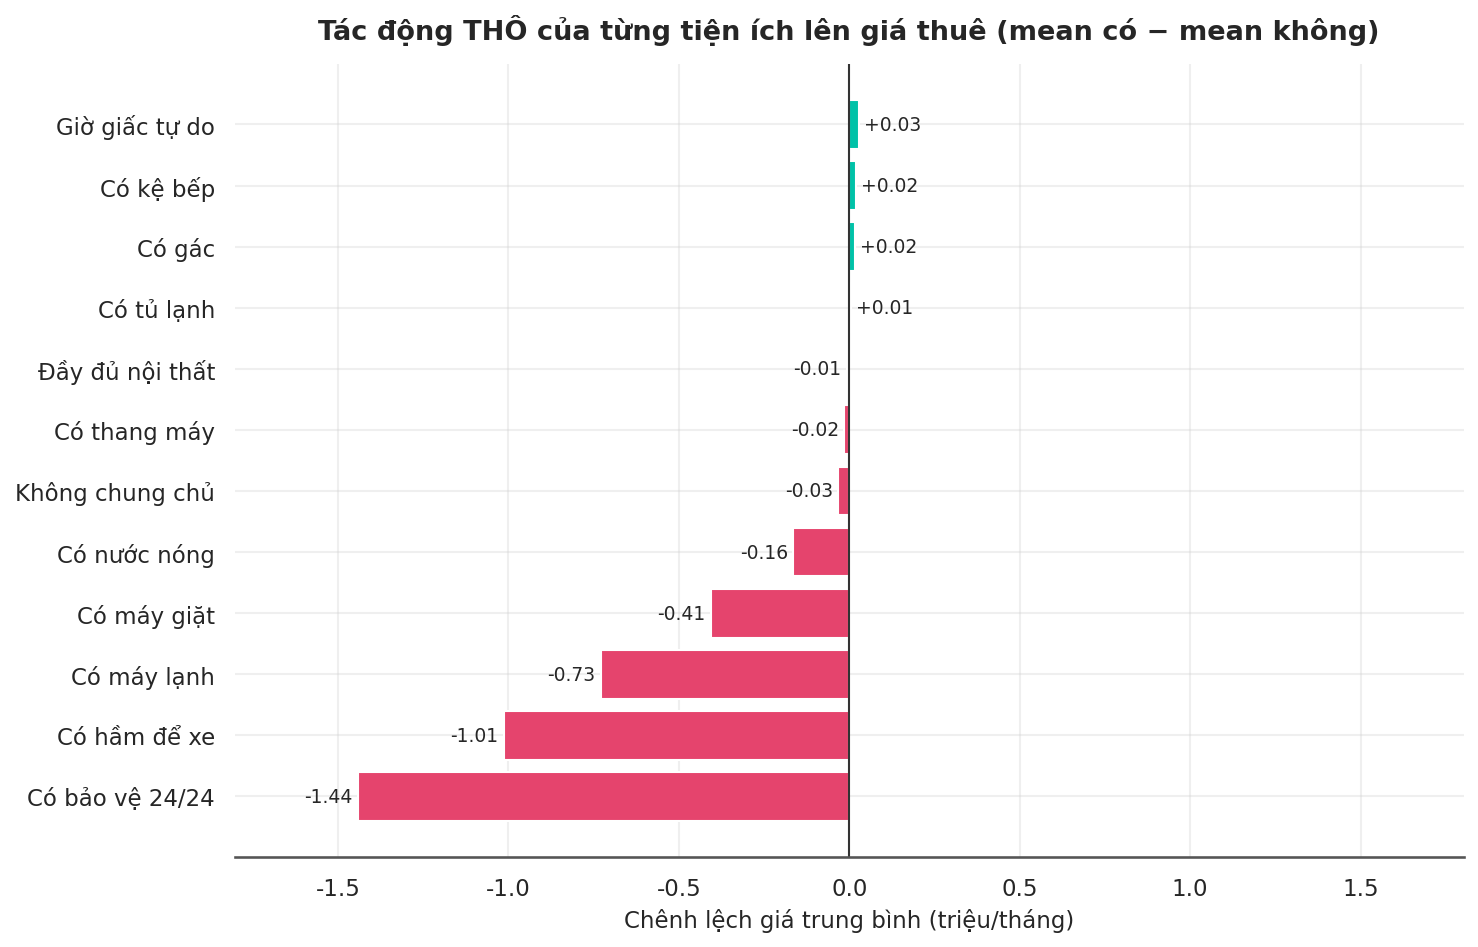
\includegraphics[width=0.86\textwidth]{eda_08_amenity_price_uplift}
  \caption{Chênh lệch giá \textbf{thô trong dữ liệu} khi có/không có từng tiện ích —
           phần lớn âm (phản trực giác). Lưu ý đây là thống kê mô tả dữ liệu như-nó-là,
           \textbf{không phải} hành vi mô hình triển khai. Câu hỏi ``tiện ích thực sự làm
           giảm giá, hay có nhân tố nhiễu?'' được trả lời từng phần ngay dưới đây
           (Nghịch lý Simpson) và triệt để ở Mục~\ref{subsec:audit}: confounding theo nguồn
           cộng với 7/12 cờ bị chế tác; mô hình triển khai cuối \textbf{không còn} hiệu ứng
           tiện ích âm nào (Hình~\ref{fig:audit_effects})}
  \label{fig:uplift}
\end{figure}

\subsubsection*{Điều tra: Nghịch lý Simpson do thiên lệch nguồn}

Kiểm tra tương quan \texttt{n\_features}--\texttt{price} \textbf{trong từng nguồn riêng biệt}:

\begin{table}[H]
  \centering
  \caption{Tương quan Spearman(\texttt{n\_features}, \texttt{price}) theo nguồn — Nghịch lý Simpson}
  \label{tab:simpson}
  \begin{tabular}{@{}lr@{}}
    \toprule
    \textbf{Nguồn} ($\geq$2.000 bài) &
    \textbf{Spearman(\texttt{n\_features}, \texttt{price})} \\
    \midrule
    phongtro123         & $\mathbf{+0.212}$ \\
    chothuenhadattoanvn & $+0.013$ \\
    github\_hn          & $-0.003$ \\
    github\_hcm         & $-0.007$ \\
    chothuephongtro     & $-0.039$ \\
    nhatot              & $-0.100$ \\
    \midrule
    \textbf{Toàn cục} & $\mathbf{-0.119}$ \\
    \bottomrule
  \end{tabular}
\end{table}

\begin{figure}[H]
  \centering
  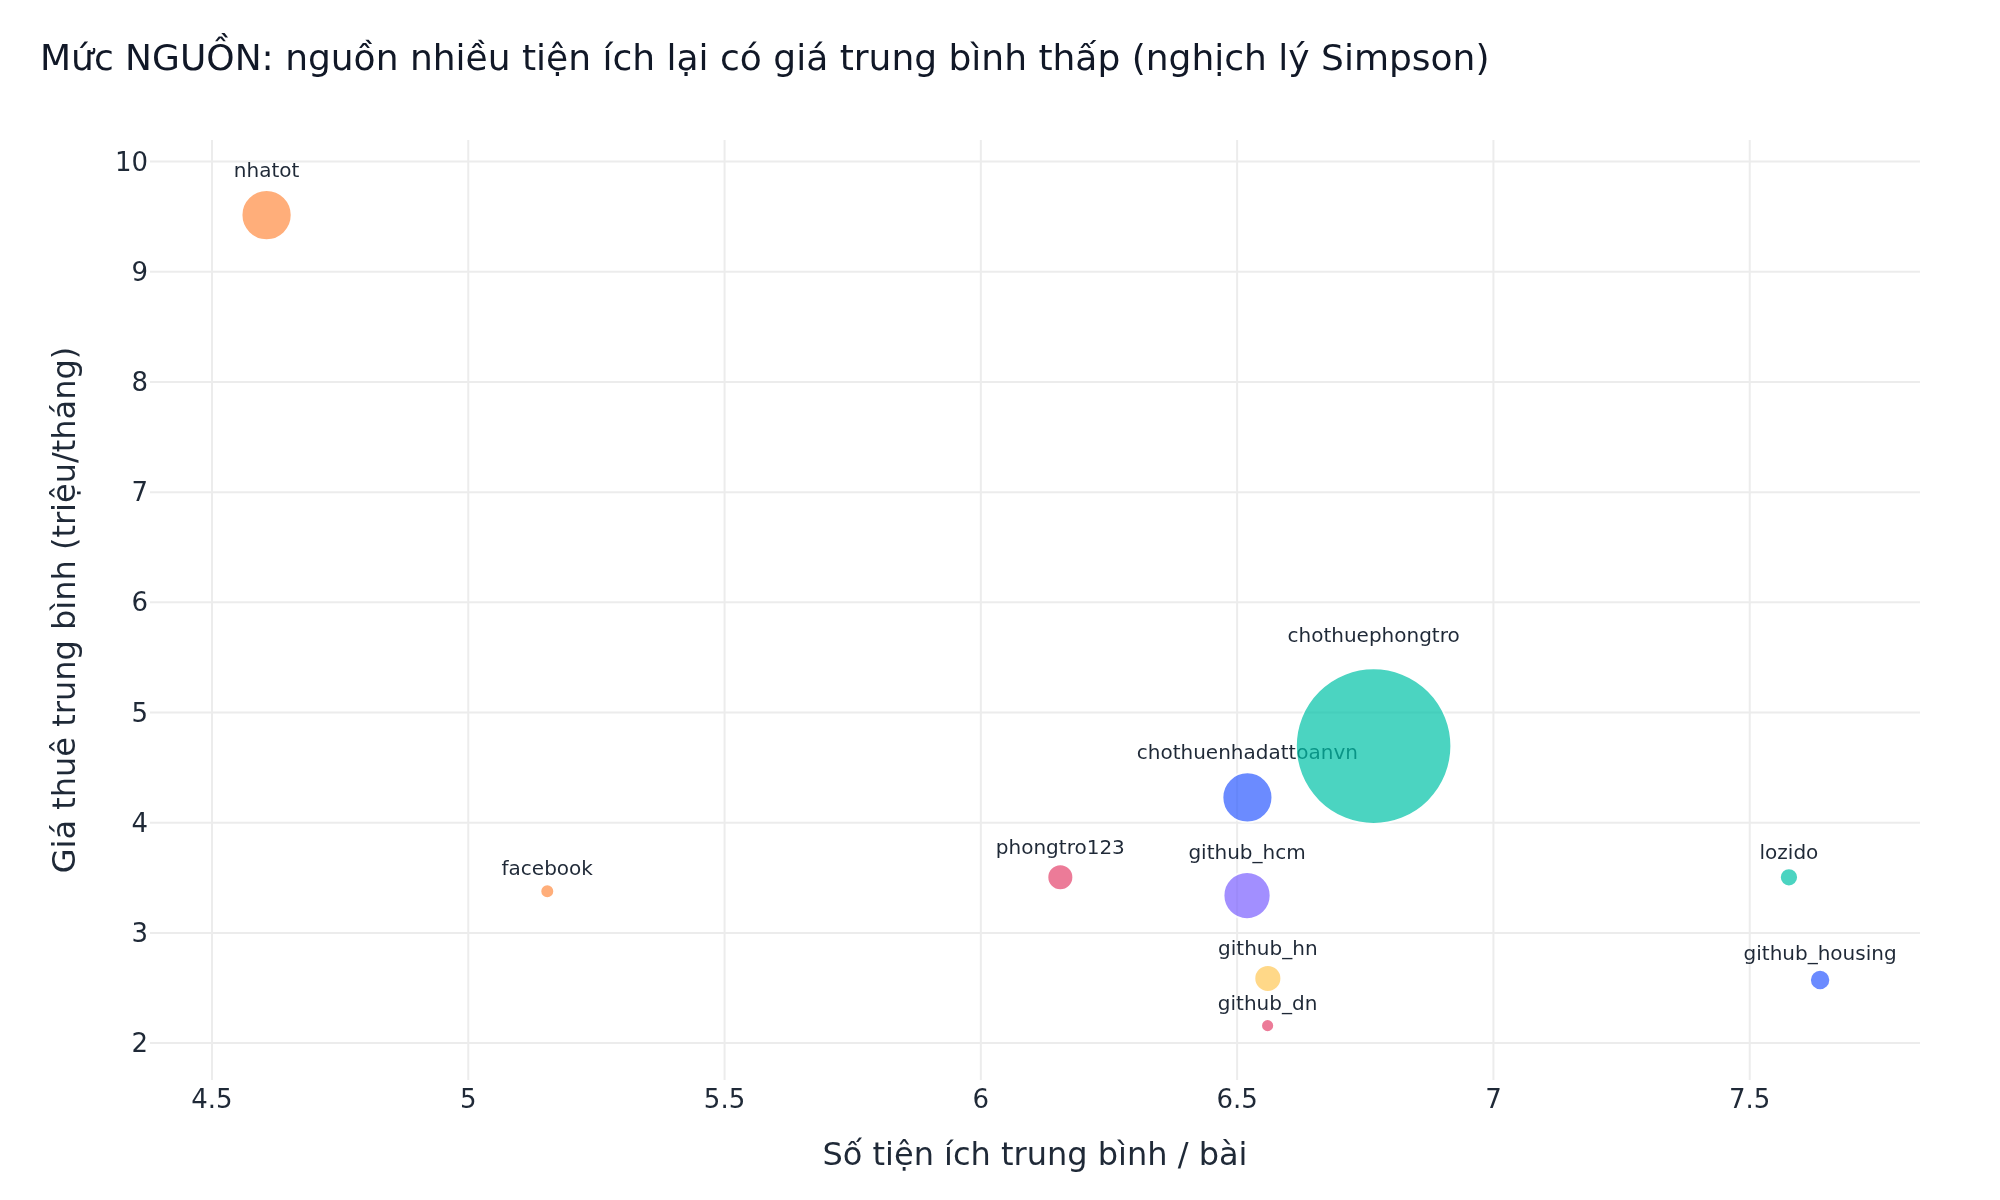
\includegraphics[width=0.86\textwidth]{eda_12_simpson_source_paradox}
  \caption{Nghịch lý Simpson: tương quan âm toàn cục do \texttt{chothuephongtro}
           (71\% dữ liệu, mặt bằng giá thấp, nhiều tiện ích) kéo trung bình xuống}
  \label{fig:simpson}
\end{figure}

\begin{quote}
  \textbf{Kết luận và quyết định thiết kế:}
  Mối tương quan âm toàn cục là do \textbf{confounding variable} — nguồn \texttt{chothuephongtro}
  chiếm 71.2\%, mặt bằng giá thấp nhưng liệt kê nhiều tiện ích.
  Hệ quả: \textbf{loại \texttt{source}} khỏi đặc trưng mô hình
  (đánh đổi một phần độ chính xác để mô hình dự báo từ đặc điểm bất động sản thật,
  không từ ``tin lấy ở web nào'').
\end{quote}

Đáng chú ý, các giá trị tương quan \textbf{gần như bằng 0 tuyệt đối} ở nhiều nguồn
(\texttt{chothuenhadattoanvn} $+0.013$, \texttt{github\_hn} $-0.003$, \texttt{github\_hcm}
$-0.007$) hóa ra là \textit{manh mối} của một vấn đề sâu hơn: kiểm toán sau triển khai
(Mục~\ref{subsec:audit}) phát hiện phần lớn cờ tiện ích của các nguồn này được
\textbf{điền ngẫu nhiên} ở bước tích hợp — biến ngẫu nhiên độc lập thì tương quan
bằng 0 với mọi thứ. Vì \texttt{n\_features} là tổng của 12 cờ trong đó 7 cờ là số
chế tác, biến này bị \textbf{loại khỏi đặc trưng mô hình} (vẫn dùng trong EDA để
mô tả dữ liệu như-nó-là).

\subsection{Feature Engineering — từ dữ liệu thô sang đặc trưng mô hình}
\label{subsec:fe}

Bước quan trọng nhất: \textbf{tách \texttt{city} và \texttt{district} từ chuỗi
\texttt{full\_address}} — đây là cách duy nhất đưa tín hiệu khu vực vào mô hình.
Thực nghiệm đối sánh (Mục~\ref{subsec:abl_fe}) xác nhận bước này là nguồn cải thiện
RMSE chính (3.5--9.4\%).

\begin{table}[H]
  \centering
  \caption{Thiết kế đặc trưng (Feature Engineering) cuối cùng — $\approx$80 chiều sau One-Hot}
  \label{tab:features}
  \begin{tabularx}{\textwidth}{@{}l X X@{}}
    \toprule
    \textbf{Nhóm} & \textbf{Đặc trưng} & \textbf{Biểu diễn} \\
    \midrule
    Số (NUM) &
      \texttt{area, bedrooms, bathrooms} &
      Chuẩn hóa Z-score
      (cần cho Ridge/LASSO; thực nghiệm~\ref{subsec:abl_fe} xác nhận) \\
    Danh mục (CAT) &
      \texttt{city, district} (tách từ \texttt{full\_address}) &
      One-Hot, gộp hạng mục hiếm (\texttt{min\_freq=100})
      $\to$ $\approx$65 chiều \\
    Nhị phân (BIN) &
      12 cờ \texttt{feature\_*} &
      0/1; ô bị chế tác $\to$ \textbf{NaN} (mask MNAR, Mục~\ref{subsec:audit}) —
      mô hình cây xử lý NaN trực tiếp, mô hình tuyến tính dùng imputer (mean) \\
    \bottomrule
  \end{tabularx}
\end{table}

\textbf{Cột bị loại có chủ đích:}
\begin{itemize}[leftmargin=*, itemsep=2pt]
  \item \texttt{source} — Nghịch lý Simpson (Mục~\ref{subsec:simpson}).
  \item \texttt{n\_features} — tổng của 12 cờ trong đó 7 cờ chế tác
        (Mục~\ref{subsec:audit}) $\Rightarrow$ phép đếm vô nghĩa,
        lại mang ``dấu vân tay nguồn''.
  \item \texttt{price\_per\_m2}, \texttt{log\_price} — rò rỉ nhãn.
  \item \texttt{posted\_date} — 46\% là giá trị sentinel.
  \item \texttt{description}, \texttt{detail\_link} — thiếu 80--96\%.
\end{itemize}

\subsection{Phân cụm K-Means và PCA}
\label{subsec:clustering}

\subsubsection*{Phân cụm K-Means ($K = 4$)}

K-Means trên (\texttt{price, area, n\_features}) chuẩn hóa, chọn $K=4$
bằng phương pháp Elbow + Silhouette.
\textbf{Ý nghĩa ra quyết định:} 4 phân khúc tương ứng với 4 đối tượng
người dùng khác nhau trong app demo (phòng bình dân, phổ thông, khá và cao cấp).

\begin{figure}[H]
  \centering
  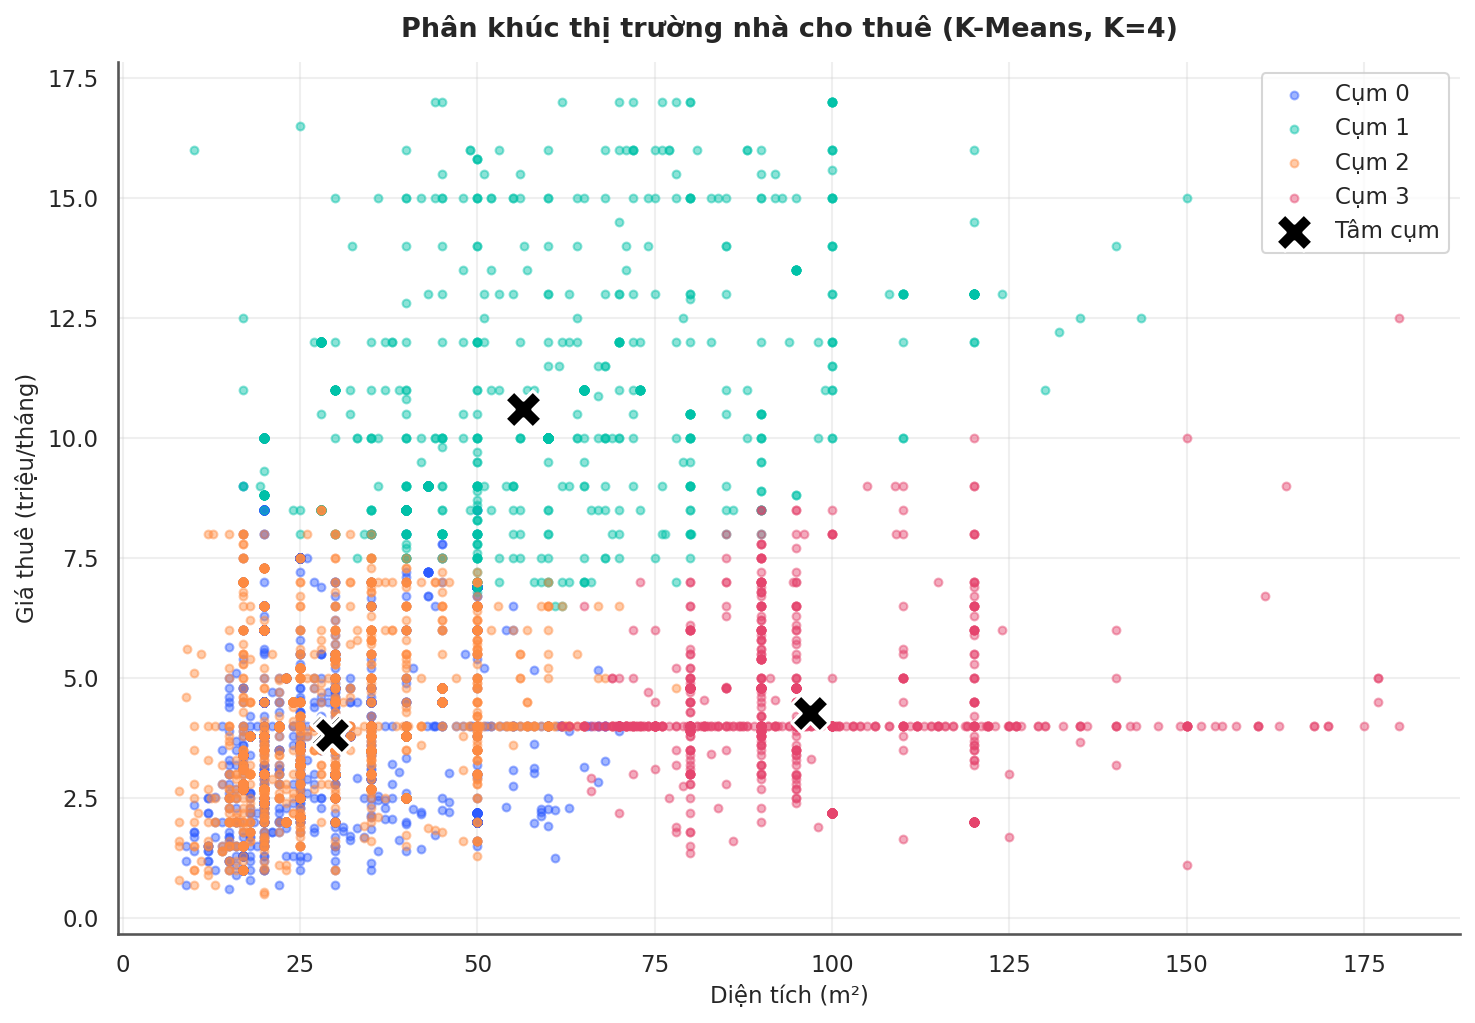
\includegraphics[width=0.86\textwidth]{eda_14_kmeans_clusters}
  \caption{4 phân khúc thị trường (K-Means, $K=4$) trên không gian
           \texttt{price} $\times$ \texttt{area}}
  \label{fig:kmeans}
\end{figure}

\subsubsection*{PCA — Cấu trúc dữ liệu}

PC1 = 36.4\%, PC2 = 21.2\%, tổng 57.6\% phương sai.
PC1 phản ánh ``quy mô'' (diện tích + số phòng + giá cùng tăng).
\textbf{Ý nghĩa:} cấu trúc tuyến tính còn lại (42.4\% phương sai chưa giải thích bởi 2 PC)
gợi ý quan hệ phi tuyến giữa khu vực và giá — lý do cần thử mô hình cây.

\begin{figure}[H]
  \centering
  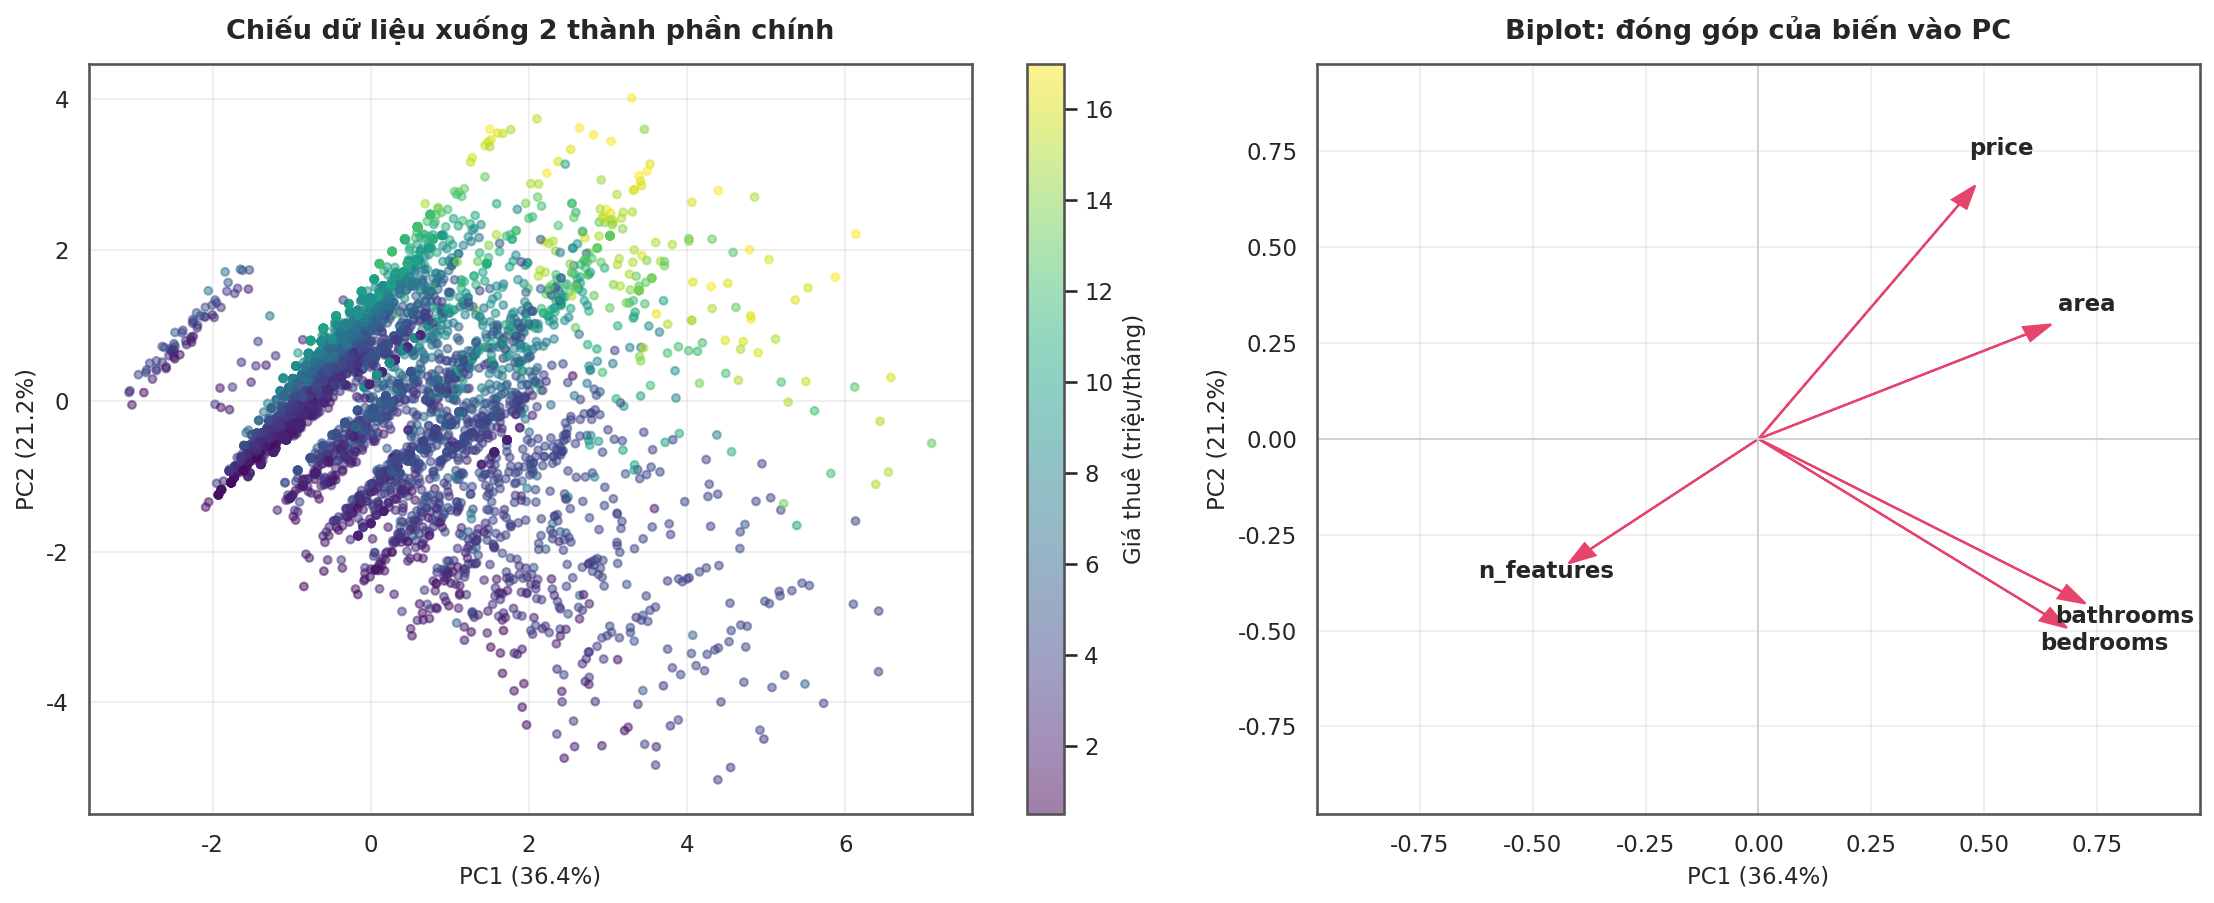
\includegraphics[width=0.80\textwidth]{eda_15_pca_2d_biplot}
  \caption{PCA 2D + Biplot: PC1 = 36.4\%, PC2 = 21.2\% — cấu trúc tuyến tính rõ nhưng
           chưa đủ giải thích toàn bộ phương sai; mô hình phi tuyến cần thiết}
  \label{fig:pca}
\end{figure}

\subsection{Bộ dữ liệu cuối (Final Data)}

Sau toàn bộ pipeline xử lý:
\begin{itemize}[leftmargin=*, itemsep=2pt]
  \item \textbf{133.586 bản ghi}; đặc trưng mô hình gồm 3 biến số + 2 biến danh mục
        (\texttt{city}/\texttt{district} tách từ FE) + 12 cờ tiện ích
        (đã mask MNAR — Bảng~\ref{tab:features}).
  \item Chia Train/Validation/Test = \textbf{70/15/15} (93.563 / 19.985 / 20.038 bản ghi).
  \item Tập Test giữ kín từ đây, chỉ dùng \textbf{đúng 1 lần} ở Mục~\ref{sec:eval}.
\end{itemize}
